\documentclass[11pt]{article}
\pdfinfoomitdate=1
\pdftrailerid{}
\pdfsuppressptexinfo=15
\usepackage[T1]{fontenc}
\usepackage[utf8]{inputenc}
\usepackage{lmodern}
\usepackage[margin=1in]{geometry}
\usepackage{amsmath,amssymb,amsthm,mathtools}
\usepackage{enumitem,booktabs}
\usepackage{tikz}
\usetikzlibrary{arrows.meta,positioning,calc,decorations.markings}
\usepackage{microtype}
\usepackage{xcolor}
\usepackage[unicode,colorlinks=true,linkcolor=blue!45!black,citecolor=blue!45!black,urlcolor=blue!45!black]{hyperref}
\usepackage[capitalise,noabbrev]{cleveref}
\hypersetup{pdftitle={Nonsingular systems of equations over arbitrary groups},pdfauthor={OpenAI}}
\newtheorem{theorem}{Theorem}
\newtheorem{lemma}{Lemma}[section]
\newtheorem{proposition}[lemma]{Proposition}
\newtheorem{corollary}[lemma]{Corollary}
\theoremstyle{definition}
\newtheorem{definition}[lemma]{Definition}
\theoremstyle{remark}
\newtheorem{remark}[lemma]{Remark}
\numberwithin{equation}{section}
\setlist{itemsep=3pt,topsep=5pt}
\setlength{\emergencystretch}{2em}
\allowdisplaybreaks[2]
\title{Nonsingular systems of equations over arbitrary groups}
\author{OpenAI}
\date{October 5, 2026}
\begin{document}
\maketitle
\begin{abstract}
Every finite nonsingular system of equations over an arbitrary group has
a simultaneous solution in an overgroup. This proves Howie's conjecture
on nonsingular systems.
\end{abstract}
\section{Introduction}
\label{sec:intro}

An equation over a group permits coefficients from that group and asks
whether the unknowns can be realized in a larger group without identifying
distinct coefficients. The exponent sums record the dependence on the
unknowns after abelianization. A system whose exponent rows are independent
is called nonsingular. We prove that every such
finite system is solvable over every coefficient group.

Let $G$ be a group and let $F_n=F(x_1,\ldots,x_n)$ be the free group on
$n$ generators. A system over $G$ consists of words
$w_1,\ldots,w_m\in G*F_n$, interpreted as equations $w_i=1$. A solution
over $G$ is a group $H$ containing an isomorphic copy of $G$, together
with elements $h_1,\ldots,h_n\in H$ at which all the words evaluate
to the identity. Define the \emph{exponent-sum matrix}
$A=(a_{ij})\in M_{m\times n}(\mathbb Z)$ by the homomorphism
\[
 G*F_n\longrightarrow\mathbb Z^n,
 \qquad G\longmapsto0,\quad x_j\longmapsto e_j:
 \qquad w_i\longmapsto(a_{i1},\ldots,a_{in}).
\]
The system is \emph{nonsingular} if $\operatorname{rank}_{\mathbb Q}A=m$.
Here $\langle\!\langle w_1,\ldots,w_m\rangle\!\rangle$ denotes normal
closure in $G*F_n$.

\begin{theorem}[Nonsingular systems]\label{thm:main}
Let $G$ be any group, let $1\le m\le n$ be integers, and let
$w_1,\ldots,w_m\in G*F_n$. If their exponent-sum matrix has row rank
$m$ over $\mathbb Q$, then the canonical homomorphism
\[
 G\longrightarrow
 (G*F_n)/\langle\!\langle w_1,\ldots,w_m\rangle\!\rangle
\]
is injective. Equivalently, the system has a simultaneous solution in
an overgroup of $G$.
\end{theorem}

The equivalence follows from the universal property of the displayed
quotient. If the canonical map is injective, the quotient itself supplies
the overgroup and the images of the free generators supply the solution.
Conversely, any solution induces a homomorphism from the quotient whose
restriction to $G$ is injective. Thus solving the equations amounts to
showing that their normal closure kills no nonidentity element of $G$.
Theorem~\ref{thm:main} imposes no countability, finiteness, or torsion
condition on $G$. The same conclusion for arbitrary sets of equations
and variables with independent exponent rows follows by a finite-relation
argument in Remark~\ref{rem:infinite-systems}.

\subsection{History and significance}
The general solvability assertion for nonsingular systems is commonly
called Howie's conjecture; see \cite[Introduction]{KlyachkoMikheenkoRomankov2024}
for this formulation and terminology. Its one-equation, one-variable
case is the Kervaire--Laudenbach conjecture: a nonzero exponent sum
should guarantee coefficient injectivity. This is stronger than the
nontriviality assertion usually called the Kervaire conjecture, which
asks whether adjoining one generator and imposing one relation can
annihilate a nontrivial group. Chen explains these formulations and their
connection with high-dimensional knot groups
\cite[Section~1]{Chen2026}. Theorem~\ref{thm:main} establishes the
finite nonsingular-system assertion for arbitrary coefficient groups.

The foundational system theorem is due to Gerstenhaber and Rothaus
\cite{GerstenhaberRothaus1962}. For a square system over a compact
connected Lie group, they compute the degree of the word map from the
determinant of its exponent-sum matrix. A nonzero determinant therefore
forces surjectivity and a simultaneous solution in that Lie group.
Their finite-group theorem also produces a finite solution overgroup,
using arithmetic specialization and reduction over finite fields.
A nonsingular rectangular
system reduces to the square case by retaining columns of a nonzero
maximal minor and setting the other variables equal to the identity. Their
argument established the usefulness of compact Lie groups, cohomology,
and degree theory in a problem stated entirely in group-theoretic terms.

A different line of work uses the topology of relative presentations.
Howie proved solvability of finite independent systems over locally
indicable groups \cite[Corollary~4.2]{Howie1981}; locally indicable
means that every nontrivial finitely generated subgroup maps onto
$\mathbb Z$. Klyachko's theorem treats a single equation in one variable
over a torsion-free group when the exponent sum is $\pm1$
\cite{Klyachko1993}. This unimodular hypothesis is stronger than a
nonzero exponent sum. Chen later recovered that theorem by estimating
the complexity of surfaces in HNN extensions
\cite[Theorem~6.9]{Chen2026}. These results illustrate two complementary
sources of control: algebraic conditions on the coefficient group and
topological restrictions on diagrams witnessing a kernel element.

The compact-unitary method also passes to metric ultraproducts. Pestov
observed its application to hyperlinear groups
\cite[Corollary~10.4]{Pestov2008}, and Nitsche and Thom give the
nonsingular-system statement explicitly
\cite[Theorem~1.2 and Lemma~2.1]{NitscheThom2022}. Here a hyperlinear,
or Connes-embeddable, group is one that embeds into a metric ultraproduct
of unitary groups with their normalized Hilbert--Schmidt metrics.
Their stronger Theorem~1.3 replaces nonsingularity by vanishing second
homology of a covering of the presentation complex obtained after
deleting the coefficients. For the presentation complex itself,
vanishing second homology is precisely independence of the exponent
rows. Their covering criterion therefore reaches beyond nonsingular
systems while retaining the hypothesis on the coefficient group.

Other developments control the solution overgroup more closely.
Klyachko, Mikheenko, and Roman'kov obtain solutions within specified
classes of solvable groups with suitable torsion-free abelian factors
\cite{KlyachkoMikheenkoRomankov2024}. Ramirez-C\^ot\'e and Wise use
the Banach fixed-point theorem for groups embedded in Magnus-type
power-series groups; their nonsingular-system construction inverts the
determinant in the coefficient ring
\cite[Theorems~9--10]{RamirezCoteWise2025}. Such conclusions address
additional structure beyond existence in an arbitrary overgroup.

The direct antecedent of our proof is the spectral-phase and planar
argument in \emph{The Kervaire theorem for groups}
\cite[Lemma~2.1, Lemma~3.1, and Theorem~4.1]{OpenAIKervaire2026}.
Its fixed-plane incidence construction treats one unimodular relator.
The extension below uses products of unitary groups and rational
intersection classes to accommodate several relator types with
different multiplicities. The cohomological background is classical
\cite{Borel1953}; related geometry of unitary eigenvalue strata and
their intersection classes is developed by Nicolaescu
\cite{Nicolaescu2010}. In finite dimensions, spectral-phase
subadditivity also follows from Thompson's exponential formula
\cite{Thompson1986}. Antezana, Larotonda, and Varela prove an
approximate version, in operator norm, for embeddable $\mathrm{II}_1$ factors
\cite[Theorem~4.4]{AntezanaLarotondaVarela2012}. Our argument instead
uses the faithful trace of the group von Neumann algebra
\cite[Section~3.3]{Jones2009} and proves the required phase inequality
directly, so the coefficients need no unitary approximation hypothesis.


\subsection{Proof and technical contribution}

The proof passes from a possible kernel relation to a planar surface.
A finite product of conjugates of the relators is represented by disks
whose boundaries read the relators or their inverses. Rectangular bands
pair occurrences of the same variable with opposite signs. The remaining
boundary arcs carry only coefficients from $G$. The key assertion is a
boundary obstruction: on a connected planar surface of this form, if all
but one boundary words are trivial in $G$, then the last is trivial as
well. Removing the innermost components then proves injectivity.

Two independent estimates establish the obstruction. First, full row rank
forces equal numbers of positive and negative disks of each relator type.
Suppose these numbers are $k_i$ for the types present. A topological
argument supplies unitary matrices mixing the $k_i$ copies of each type
so that a finite-dimensional unitary matrix has at least $2\sum_i k_i$ fixed
directions. Second, a spectral-phase function measures the boundary words
through the left regular representation of $G$. Its subadditivity turns
the fixed-space estimate into an upper bound. A direct calculation around
the boundary circles attains that bound plus a nonnegative term measuring
the possibly nontrivial boundary word. Euler characteristic makes the
two constants agree, and faithfulness of the trace forces that word to
be the identity.

The spectral-phase and planar-surface strategy comes from the
one-relator unimodular theorem in~\cite{OpenAIKervaire2026}. We give
the required arguments in full. The principal extension is the
multi-block fixed-space theorem in Section~\ref{sec:fixed}. It concerns
block matrices built from independent unitary variables of possibly
different sizes, followed by arbitrary fixed unitary matrices. Full row
rank of the signed block-multiplicity matrix forces a simultaneous lower
bound on the dimensions of their fixed spaces. The proof pairs
fixed-subspace incidence cycles with the product of the unitary-variable
groups. Only the maximal-length exterior terms in cohomology contribute;
their coefficient is a product of nested nonzero minors. This makes
rational nonsingularity sufficient and gives an intersection principle
that is independent of its application to equations over groups.

Section~\ref{sec:phase} establishes the phase inequality in the finite
operator algebra of the left regular representation and computes the
phase of a weighted cyclic shift. Section~\ref{sec:planar} combines
these results to prove the boundary obstruction. Section~\ref{sec:kernel}
constructs the planar surfaces from an arbitrary kernel relation and
completes the proof. The unitary topology is used only for finite complex
matrices on the copy indices; the group coefficients are retained as
operators throughout. This separation allows the argument to apply to
arbitrary coefficient groups.

\section{Simultaneous fixed spaces}\label{sec:fixed}

The rank hypothesis enters the proof through the following finite-dimensional
statement.  A unitary matrix may occur in several blocks, with either exponent
$1$ or exponent $-1$.  Only the signed numbers of its occurrences matter for
the lower bound on the total fixed-space dimension.
The proof extends the single-matrix incidence argument of
\cite[Lemma~3.1]{OpenAIKervaire2026} by using rational cohomology and
nested nonzero minors to accommodate several unitary matrix variables.

\begin{theorem}[Simultaneous fixed spaces]\label{thm:fixed-space}
Let $r\geq 0$ and $n\geq 1$, and let $k_1,\ldots,k_r$ be positive integers.
For each $j\in\{1,\ldots,n\}$, let $\mathcal B_j$ be a finite ordered list
of pairs $(i,s)$ with $1\leq i\leq r$ and $s\in\{1,-1\}$; repetitions
are allowed.  Set
\[
 d_j=\sum_{(i,s)\in\mathcal B_j}k_i,
 \qquad
 b_{ij}=\sum_{\substack{(i',s)\in\mathcal B_j\\i'=i}}s,
 \qquad B=(b_{ij}).
\]
Suppose that $B$ has row rank $r$ over $\mathbb Q$.  For arbitrary
$P_j\in\mathrm U(d_j)$, define
\[
 D=\prod_{i=1}^r\mathrm U(k_i),
 \qquad
 F_j(X)=\operatorname{diag}_{(i,s)\in\mathcal B_j}(X_i^s)P_j
 \quad (X\in D).
\]
Then there is $X\in D$ such that
\begin{equation}\label{eq:fixed-space-bound}
 \sum_{j=1}^n\dim_{\mathbb C}\ker(F_j(X)-I_{d_j})
 \ \geq\ \sum_{i=1}^r k_i.
\end{equation}
Here $\mathrm U(0)$ and an empty product of groups are points, and the
fixed-space dimension in dimension zero is zero.
\end{theorem}

\begin{proof}
\emph{Choosing target dimensions.}
The case $r=0$ is immediate.  Assume $r>0$, and reorder the rows so that
$k_1\geq\cdots\geq k_r$.  We first allocate the desired fixed-space
dimensions among the maps $F_j$.  There are distinct columns
$j_1,\ldots,j_r$ such that
\begin{equation}\label{eq:fixed-nested-minors}
 \det B[1,\ldots,t\mid j_1,\ldots,j_t]\ne 0
 \qquad (1\leq t\leq r).
\end{equation}
Indeed, the first $t$ rows have rank $t$.  The columns chosen at the previous
step remain independent on these rows, since their restrictions to the
first $t-1$ rows are independent; they can therefore be extended by one
column.  Define
\[
 l_{j_t}=k_t\quad(1\leq t\leq r),
 \qquad l_j=0\quad\text{for unchosen columns}.
\]
These choices satisfy $l_j\leq d_j$.  To see this for $j=j_t$, the
nonzero minor in \eqref{eq:fixed-nested-minors} implies that $b_{i,j_t}\ne0$
for some $i\leq t$.  The list $\mathcal B_{j_t}$ thus contains a block
of size $k_i\geq k_t$.  Moreover,
\begin{equation}\label{eq:fixed-target-dimensions}
 \sum_j l_j=\sum_i k_i,
 \qquad \sum_j l_j^2=\sum_i k_i^2=\dim_{\mathbb R}D.
\end{equation}
We will obtain $\dim\ker(F_j(X)-I_{d_j})\geq l_j$ simultaneously.
The equality of dimensions in \eqref{eq:fixed-target-dimensions} makes
this an intersection problem of complementary dimensions.  We develop
the cohomology classes that detect the required intersection.

\smallskip\noindent
\emph{Primitive cohomology classes.}
All cohomology in this proof has coefficients in $\mathbb Q$.  The
classical computation of unitary-group cohomology
\cite[Proposition~9.1 and Sections~19--20]{Borel1953} gives generators
\begin{equation}\label{eq:fixed-unitary-cohomology}
 H^*(\mathrm U(d);\mathbb Q)
   =\Lambda(e_{1,d},\ldots,e_{d,d}),
 \qquad |e_{a,d}|=2a-1,
\end{equation}
where $\Lambda$ denotes the exterior algebra.  Compatibility means that
inclusion as a coordinate block, with the identity on its complement,
satisfies
\begin{equation}\label{eq:fixed-block-restriction}
 \iota_{k,d}^*e_{a,d}=
 \begin{cases}
 e_{a,k},&a\leq k,\\
 0,&a>k.
 \end{cases}
\end{equation}
We will choose the generators to satisfy this compatibility and to be
\emph{primitive}: if $\mu$ is group multiplication, then
\begin{equation}\label{eq:fixed-primitivity}
 \mu^*e_{a,d}=e_{a,d}\otimes1+1\otimes e_{a,d}.
\end{equation}
Thus these classes add under multiplication, just as degree-one
classes do on a torus.

For completeness, these properties follow together from the last-column
bundle
\[
 \mathrm U(d-1)\longrightarrow\mathrm U(d)
       \longrightarrow S^{2d-1}.
\]
Start with the degree-one generator of $\mathrm U(1)=S^1$.  For $d\geq2$,
the base is simply connected, so the coefficient system in the
multiplicative Serre spectral sequence is constant
\cite[Theorem~5.2 and Section~5.3]{McCleary2001}.  Its second page is
\[
 E_2^{p,q}=H^p(S^{2d-1};\mathbb Q)
              \otimes H^q(\mathrm U(d-1);\mathbb Q).
\]
Its only nonzero columns are $p=0,2d-1$.  The only possible differential
between them is $d_{2d-1}$, which sends fiber degree $q$ to degree
$q-2d+2$.  Each fiber generator has degree at most $2d-3$, so its
differential has negative target degree and vanishes.
The differential vanishes on all their products by the
product rule for the differential.  Consequently the spectral sequence
collapses.  Its edge maps show that restriction to $\mathrm U(d-1)$ is
an isomorphism in degrees below $2d-1$, and that the pullback of the sphere's
top class is nonzero.  Lift each earlier generator in its degree, and take
this sphere pullback as $e_{d,d}$.  Their exterior products give the basis
in \eqref{eq:fixed-unitary-cohomology}: they give that basis in the
associated graded algebra supplied by the spectral sequence, and their
squares vanish because they have odd degree and the coefficients are
rational.  This also proves compatibility with the standard inclusions.

To check primitivity, subtract the two summands on the right of
\eqref{eq:fixed-primitivity} from its left side.  The difference restricts
to zero on either factor at the identity, so every term in its K\"unneth
decomposition has positive degree in both factors.  Each such degree is
at most $2d-2$.  Restriction to
$\mathrm U(d-1)\times\mathrm U(d-1)$ is injective on all these
bidegrees, by the edge-map isomorphism just proved.  On this product the
difference vanishes: for $a<d$ this is the induction hypothesis, and for
$a=d$ it follows because $e_{d,d}$ is pulled back by the last-column
projection, which is constant on the fiber.
This proves \eqref{eq:fixed-primitivity}; the case $d=1$ is immediate.
Coordinate-block inclusions in other positions are conjugate to the
standard one, and conjugation is homotopic to the identity in the
connected group $\mathrm U(d)$.  Finally, inversion sends $e_{a,d}$
to $-e_{a,d}$, by pulling \eqref{eq:fixed-primitivity} back along
$X\mapsto(X,X^{-1})$.

\smallskip\noindent
\emph{The fixed-space incidence class.}
We next construct a class that detects a fixed space of dimension at
least $l$, for $0\leq l\leq d$.  Let
\[
 R(d,l)=\{(W,E): W\in\mathrm U(d),\ E\in
        \operatorname{Gr}_l(\mathbb C^d),\ W|_E=I_E\},
 \qquad p(W,E)=W,
\]
where $\operatorname{Gr}_l(\mathbb C^d)$ is the complex Grassmannian of
$l$-dimensional subspaces.  Over a subspace $E$, the possible $W$ are
precisely the unitary transformations of $E^\perp$, extended by the
identity on $E$.  Orthonormal frame charts therefore make $R(d,l)$ a
smooth bundle over the Grassmannian with fiber $\mathrm U(d-l)$.
It is compact and without boundary, and
\[
 \dim_{\mathbb R}R(d,l)=2l(d-l)+(d-l)^2=d^2-l^2.
\]
The complex orientation of the Grassmannian and an orientation of
$\mathrm U(d-l)$ orient this bundle: changes of frame act on the fiber
by conjugation and preserve orientation.  Choose orientations and let
\[
 \alpha(d,l)=\operatorname{PD}\bigl(p_*[R(d,l)]\bigr)
        \in H^{l^2}(\mathrm U(d);\mathbb Q).
\]
Here $\operatorname{PD}$ is Poincar\'e duality
\cite[Theorem~3.30]{Hatcher2002}.  It applies to the
homology class pushed forward by $p$; the image of $p$ need not itself be
a submanifold.  Its image consists exactly of those $W$ with
$\dim\ker(W-I_d)\geq l$.

We recall the geometric interpretation of this class.  If $M$ is a
closed oriented manifold of dimension $l^2$ and $f:M\to\mathrm U(d)$,
then $\langle f^*\alpha(d,l),[M]\rangle$ is the intersection number of
$f$ and $p$.  When these maps are transverse, it is the signed count of
pairs $(x,(W,E))$ with $f(x)=p(W,E)$.  This follows by intersecting
$f\times p$ with the diagonal of $\mathrm U(d)\times\mathrm U(d)$:
transversality makes its inverse image a compact oriented zero-manifold,
whose signed count gives the intersection pairing.
In particular, disjoint images give intersection number zero: disjoint
maps from compact manifolds have disjoint sufficiently small transverse
perturbations.  The same interpretation holds for products of these
maps and classes.

The part of $\alpha(d,l)$ we need is
\begin{equation}\label{eq:fixed-incidence-leading-term}
 \alpha(d,l)=c_{d,l}e_{1,d}\cdots e_{l,d}
       +\text{terms with fewer than $l$ generators},
 \qquad c_{d,l}\ne0.
\end{equation}
For $l=0$, the map $p$ is the identity and we take
$\alpha(d,0)=1$ and $c_{d,0}=1$.
For $l>0$, a product of $u$ distinct generators has degree at least
$1+3+\cdots+(2u-1)=u^2$.  Since $\alpha(d,l)$ has degree $l^2$, its
expansion contains at most $l$ generators in each term, and the sole
possible term of length $l$ is the one displayed in
\eqref{eq:fixed-incidence-leading-term}.

To show that its coefficient is nonzero, consider
\[
 f:\mathrm U(l)\longrightarrow\mathrm U(d),
 \qquad f(X)=X\oplus(-I_{d-l}).
\]
There is exactly one intersection pair for $f$ and $p$: it has
$X=I_l$, $W=W_0=I_l\oplus(-I_{d-l})$, and $E=E_0=\mathbb C^l\oplus0$.
Indeed, the second summand has no fixed vectors, while an $l$-dimensional
fixed space in the first summand forces $X=I_l$.  This intersection is
transverse.  Identify the tangent space at $W_0$ with skew-Hermitian
matrices by right multiplication by $W_0^{-1}$.  Variations of $f$ fill
the upper-left block; variations of $p$ in the fiber over $E_0$ fill
the lower-right block.  For a linear map $Z:E_0\to E_0^\perp$, put
\[
 T=\begin{pmatrix}0&-Z^*\\ Z&0\end{pmatrix}.
\]
The path $(e^{tT}W_0e^{-tT},e^{tT}E_0)$ lies in $R(d,l)$ and its image
under $p$ has tangent vector
\[
 [T,W_0]W_0^{-1}=2T.
\]
These vectors supply every off-diagonal direction.  The unique
intersection therefore has multiplicity $1$ or $-1$.  The map $f$ is
homotopic to the coordinate inclusion, so
\eqref{eq:fixed-block-restriction} computes its pullback.  Terms with
an index above $l$ vanish; any remaining term with fewer than $l$
generators has degree less than $\dim\mathrm U(l)=l^2$.  Only the
displayed term in \eqref{eq:fixed-incidence-leading-term} can account for
the nonzero intersection number, proving $c_{d,l}\ne0$.
The same argument includes $l=d$, when the complementary blocks are
absent.

\smallskip\noindent
\emph{Computing the intersection number.}
We now apply these classes to the maps in the statement.  Write
$e_{a,k_i}^{(i)}$ for the generator pulled back from the $i$th factor of
$D$.  Primitivity, compatibility with block inclusions, and the inversion
formula give
\begin{equation}\label{eq:fixed-generator-pullback}
 F_j^*e_{a,d_j}
   =\sum_{i:\,k_i\geq a}b_{ij}e_{a,k_i}^{(i)}
       \qquad(1\leq a\leq d_j).
\end{equation}
To justify the use of multiplication here, write a block diagonal map
as the product of maps that act on one block and are the identity on
all others.  Each positive occurrence contributes one generator and
each negative occurrence its negative.  Right multiplication by $P_j$
is homotopic to the identity and has no effect on cohomology.

Consider the top-degree class
\[
 \Omega=\prod_{j=1}^nF_j^*\alpha(d_j,l_j)
       \in H^{\sum_i k_i^2}(D;\mathbb Q).
\]
The exterior algebra $H^*(D;\mathbb Q)$ has altogether $\sum_i k_i$
generators, all of positive degree.  A nonzero monomial of top degree
must contain every one of them.  By
\eqref{eq:fixed-generator-pullback}, pullback preserves the number of
generators in each term, unless that term vanishes.  It follows that
any use of a shorter term from
\eqref{eq:fixed-incidence-leading-term} contributes zero to $\Omega$.
Thus we need only compute the product of the displayed leading terms.

For each $a\in\{1,\ldots,k_1\}$, put
$t_a=|\{i:k_i\geq a\}|$.  The rows with $k_i\geq a$ are
$1,\ldots,t_a$, and the selected columns with $l_j\geq a$ are
$j_1,\ldots,j_{t_a}$.  Grouping the exterior factors of degree $2a-1$
together gives
\[
 \prod_{t=1}^{t_a}
   \left(\sum_{i=1}^{t_a}b_{i,j_t}e_{a,k_i}^{(i)}\right)
 =\det B[1,\ldots,t_a\mid j_1,\ldots,j_{t_a}]
       \prod_{i=1}^{t_a}e_{a,k_i}^{(i)}.
\]
Consequently the coefficient of the top monomial in $\Omega$, up to
an overall sign, is
\begin{equation}\label{eq:fixed-top-coefficient}
 \left(\prod_{j=1}^n c_{d_j,l_j}\right)
 \prod_{a=1}^{k_1}
   \det B[1,\ldots,t_a\mid j_1,\ldots,j_{t_a}].
\end{equation}
Every factor is nonzero, by
\eqref{eq:fixed-nested-minors} and
\eqref{eq:fixed-incidence-leading-term}.  Hence
$\langle\Omega,[D]\rangle\ne0$.

Finally, let $F=(F_1,\ldots,F_n)$ and let
$p_{\mathrm{tot}}=\prod_j p$ be the map from
$\prod_jR(d_j,l_j)$ to $\prod_j\mathrm U(d_j)$.
Up to the harmless orientation sign, $\Omega$ is the pullback by $F$
of the Poincar\'e dual of the cycle defined by $p_{\mathrm{tot}}$.
Its nonzero evaluation implies that these two maps have intersecting
images.  At an intersection, $F_j(X)$ fixes an $l_j$-plane for every
$j$, which gives \eqref{eq:fixed-space-bound} by
\eqref{eq:fixed-target-dimensions}.
\end{proof}

\section{Spectral phase}\label{sec:phase}

The planar argument will associate unitary operators to the boundary circles
of a surface.  We need a nonnegative numerical invariant that detects the
identity, is subadditive under multiplication, and can be calculated on a
weighted cyclic shift.  We develop these properties in the operator algebra
of an arbitrary group, following the spectral-phase argument of
\cite[Lemma~2.1 and Section~4.3]{OpenAIKervaire2026}.

\subsection{The trace and the choice of phase}

Let $G$ be any group, and let $\{\delta_x:x\in G\}$ be the standard
orthonormal basis of $\ell^2(G)$.  Define left and right translations by
\[
 L(a)\delta_x=\delta_{ax},\qquad
 R_a\delta_x=\delta_{xa^{-1}}.
\]
They commute.  We work in the von Neumann algebra
\[
 \mathcal M=\{T\in\mathcal B(\ell^2(G)):TR_a=R_aT
             \text{ for every }a\in G\},
\]
which contains every $L(a)$.  For a positive integer $d$, regard
$M_d(\mathcal M)$ as operators on $\mathbb C^d\otimes\ell^2(G)$ and set
\begin{equation}\label{eq:group-trace}
 \tau_d(T)=\sum_{j=1}^d(T_{jj})_{1,1},\qquad \tau=\tau_1.
\end{equation}
Here $(T_{jj})_{1,1}$ is the coefficient of $\delta_1$ in
$T_{jj}\delta_1$.  The trace is \emph{unnormalized}: $\tau_d(I)=d$.
For the group von Neumann algebra and this trace construction, see
\cite[Section~3.3]{Jones2009}.

We record why this is a faithful normal trace, including when $G$ is
uncountable.  If $T\in\mathcal M$ and $T\delta_1=\sum_x t_x\delta_x$,
commutation with right translations gives
\[
 T_{x,y}=t_{xy^{-1}}.
\]
For $A,B\in\mathcal M$ with corresponding coefficient families $a,b$,
\[
 \tau(AB)=\sum_{x\in G}a_{x^{-1}}b_x
         =\sum_{x\in G}b_{x^{-1}}a_x=\tau(BA).
\]
These sums converge absolutely by Cauchy--Schwarz; each square-summable
family has countable support.  Summing over the matrix indices proves
traciality of $\tau_d$.  Positivity and normality follow from its expression
as a finite sum of vector functionals.  If $T\geq0$ and $\tau_d(T)=0$, then
\[
 0=\sum_{j=1}^d
   \bigl\|T^{1/2}(e_j\otimes\delta_1)\bigr\|^2.
\]
The square root commutes with all simultaneous right translations, so it
kills $e_j\otimes\delta_x$ for every $j,x$.  Thus $T=0$, proving
faithfulness.

The bounded Borel functional calculus of a normal operator in
$M_d(\mathcal M)$ remains in this algebra.  For a unitary $U$, its spectral
projections define a finite measure
$\mu_U(E)=\tau_d(\mathbf1_E(U))$ on the unit circle $\mathbb T$, and
\begin{equation}\label{eq:phase-spectral-integral}
 \tau_d(f(U))=\int_{\mathbb T}f\,d\mu_U,
 \qquad \mu_U(\mathbb T)=d.
\end{equation}
In particular, uniformly bounded pointwise convergence of Borel functions
implies convergence of these trace evaluations.

Choose the phase with its cut at $1$ by
\begin{equation}\label{eq:phase-definition}
 h(e^{2\pi i t})=t-\lfloor t\rfloor,\qquad
 \ell(U)=\tau_d(h(U)).
\end{equation}
Thus $h(1)=0$, and $h$ is right-continuous in the angle.  Since
$h(U)\geq0$ and $U=\exp(2\pi i h(U))$, faithfulness gives
\begin{equation}\label{eq:phase-faithful}
 \ell(U)\geq0,\qquad \ell(U)=0\ \Longleftrightarrow\ U=I.
\end{equation}
The phase is invariant under unitary conjugation and additive on direct
sums.  On scalar matrices, viewed as matrices over $\mathcal M$, it is the
sum of the phases of the eigenvalues, counted with multiplicity.

\subsection{Subadditivity}

\begin{lemma}[Spectral-phase subadditivity]\label{lem:phase-subadditivity}
For every group $G$, every positive integer $d$, and all unitaries
$U,V\in M_d(\mathcal M)$,
\[
 \ell(UV)\leq\ell(U)+\ell(V).
\]
\end{lemma}

\begin{proof}
Put $D=h(V)$ and join $U$ to $UV$ by the unitary path
\[
 W_u=Ue^{2\pi i uD},\qquad 0\leq u\leq1.
\]
We first calculate the change of a smooth function along this path, and
then approximate the discontinuous function $h$ from the correct side of
its cut.  For $f\in C^\infty(\mathbb T)$ write
$f'(e^{2\pi it})=\frac{d}{dt}f(e^{2\pi it})$.  We claim that
\begin{equation}\label{eq:phase-derivative}
 \frac{d}{du}\tau_d(f(W_u))=\tau_d(f'(W_u)D).
\end{equation}
Indeed, $W'_u=2\pi iW_uD$.  The product and inverse rules, followed by
cyclic permutation inside the trace, give for every integer $k$
\[
 \frac{d}{du}\tau_d(W_u^k)=2\pi i k\,\tau_d(W_u^kD).
\]
This proves \eqref{eq:phase-derivative} for Laurent polynomials.  For smooth
$f$, its Fourier coefficients satisfy
$\sum_{k\in\mathbb Z}(1+|k|)|\widehat f(k)|<\infty$, while
$\|\frac{d}{du}W_u^k\|\leq2\pi|k|\|D\|$.  Thus the Fourier series and
its differentiated series converge uniformly in operator norm, proving
\eqref{eq:phase-derivative} in general.

If $f$ is real-valued and $f'\leq1$, then $I-f'(W_u)\geq0$.  Although
$D$ need not commute with $W_u$, traciality gives the required inequality:
\[
 \tau_d(D)-\tau_d(f'(W_u)D)
 =\tau_d\bigl(D^{1/2}(I-f'(W_u))D^{1/2}\bigr)\geq0.
\]
Integration of \eqref{eq:phase-derivative} therefore yields
\begin{equation}\label{eq:phase-smooth-bound}
 \tau_d(f(UV))-\tau_d(f(U))\leq\tau_d(D).
\end{equation}

For $0<\varepsilon<1$, choose a nonnegative smooth function
$\rho_\varepsilon$ supported in $(0,\varepsilon)$ with integral one, and
define
\[
 f_\varepsilon(e^{2\pi it})
 =\int_0^\varepsilon
   \rho_\varepsilon(s)h(e^{2\pi i(t+s)})\,ds.
\]
This is a smooth function on the circle, with $0\leq f_\varepsilon\leq1$.
For $\delta>0$ the fractional-part function satisfies
\[
 h(e^{2\pi i(t+\delta)})-h(e^{2\pi it})\leq\delta.
\]
Averaging this inequality and taking the difference quotient shows that
$f'_\varepsilon\leq1$.  Right-continuity gives
$f_\varepsilon(\lambda)\to h(\lambda)$ for every $\lambda\in\mathbb T$.
At the cut this follows explicitly from
$0\leq f_\varepsilon(1)\leq\varepsilon$; symmetric smoothing would not
have this property.  Apply \eqref{eq:phase-smooth-bound} to
$f_\varepsilon$ and pass to the limit by
\eqref{eq:phase-spectral-integral}.  Since $\tau_d(D)=\ell(V)$, the
result is the stated inequality.
\end{proof}

The same right-continuity also gives, for any fixed $c\geq0$,
\begin{equation}\label{eq:phase-right-limit}
 \lim_{\varepsilon\downarrow0}
 \ell(e^{2\pi i c\varepsilon}U)=\ell(U).
\end{equation}
In the opposite direction the identity has a jump:
$\ell(e^{-2\pi i\varepsilon}I_d)=d(1-\varepsilon)$ for
$0<\varepsilon<1$.  These two behaviors at the cut will distinguish the
possibly nontrivial boundary circle from the trivial ones in the planar
argument.

\subsection{The phase of a weighted cycle}

Subadditivity will give an upper bound on the operator associated to a
surface.  The following exact calculation will express its phase in terms
of the boundary words.

\begin{lemma}[Weighted-cycle formula]\label{lem:cycle-phase}
Let $a$ be a positive integer, let $Q_1,\ldots,Q_a\in\mathcal M$ be unitary, and define
$T\in M_a(\mathcal M)$ by
\[
 T(e_t\otimes v)=e_{t+1}\otimes Q_tv\quad(1\leq t\leq a),
 \qquad e_{a+1}=e_1.
\]
If $C=Q_aQ_{a-1}\cdots Q_1$ is the product around the cycle starting at
the first coordinate, then
\begin{equation}\label{eq:cycle-phase}
 \ell(T)=\frac{a-1}{2}+\tau(h(C)).
\end{equation}
\end{lemma}

\begin{proof}
Put $\zeta=e^{2\pi i/a}$.  Conjugating $T$ by the scalar diagonal matrix
with entries $1,\zeta,\ldots,\zeta^{a-1}$ gives $\zeta T$.  Hence
$\ell(\zeta^jT)=\ell(T)$ for every integer $j$.  The scalar identity
\[
 \sum_{j=0}^{a-1}h(\zeta^j\lambda)
 =\frac{a-1}{2}+h(\lambda^a),\qquad \lambda\in\mathbb T,
\]
follows by listing the fractional parts of the $a$ equally spaced angles;
it holds also when one of them is zero.  Applying bounded Borel functional
calculus and taking the unnormalized trace gives
\[
 a\ell(T)=\frac{a(a-1)}2+\tau_a(h(T^a)).
\]
The operator $T^a$ is diagonal.  Its first diagonal entry is $C$, and the
other entries are the products around the same cycle with different
starting coordinates.  Consecutive such products are conjugate by the
corresponding $Q_t$, so every diagonal entry has phase trace
$\tau(h(C))$.  Thus $\tau_a(h(T^a))=a\tau(h(C))$, proving
\eqref{eq:cycle-phase}.
\end{proof}

\section{The planar boundary obstruction}\label{sec:planar}

We now combine the fixed-space theorem with the phase inequality.  The
result is a statement about a planar surface assembled from copies of the
relators: if every boundary component but one reads the identity in $G$,
then the remaining component does too.  This extends the one-relator
boundary argument of \cite[Theorem~4.1 and Section~4]{OpenAIKervaire2026};
the new fixed-space input allows the different relator types to be treated
simultaneously.

Cyclically conjugating the words does not change their normal closure or
their exponent sums.  We may therefore write
\begin{equation}\label{eq:word-slots}
 w_i=x_{\nu_{i,1}}^{s_{i,1}}g_{i,1}\cdots
     x_{\nu_{i,N_i}}^{s_{i,N_i}}g_{i,N_i},
 \qquad
 g_{i,t}\in G,\quad s_{i,t}\in\{1,-1\},\quad
 1\leq \nu_{i,t}\leq n.
\end{equation}
Here each occurrence is a single variable letter, coefficients may be the
identity, and $N_i\geq1$ because the $i$th row of $A$ is nonzero.

A \emph{word disk of type $i$ and sign $+$ or $-$} is an oriented disk
whose boundary reads $w_i$ or $w_i^{-1}$, respectively.  Its variable
letters occupy disjoint closed intervals called \emph{slots}, separated
by nonempty \emph{corner arcs} carrying the coefficients.  On both signs
of disk, index the slots by the positions $t$ in \eqref{eq:word-slots}.
Indices are cyclic modulo $N_i$.  The boundary data are then
\begin{equation}\label{eq:slot-conventions}
\begin{array}{c|c|c|c}
 \text{disk sign}&\text{successor of }t&
 \text{variable at }t&\text{corner after }t\\ \hline
 +&t+1&x_{\nu_{i,t}}^{s_{i,t}}&g_{i,t}\\
 -&t-1&x_{\nu_{i,t}}^{-s_{i,t}}&g_{i,t-1}^{-1}
\end{array}
\end{equation}
The exponent $s_{i,t}$ or $-s_{i,t}$ in this table is the slot's
\emph{traversal sign}.  Attach rectangular bands to pairs of slots so
that the orientations extend across the bands.  Every slot is used once,
and paired slots must have the same variable index and opposite traversal
signs.  The remaining boundary consists of corner arcs and band sides;
its word in $G$ is obtained by reading the corner labels, with no label
contributed by a band side.  Changing the starting corner conjugates this
word, so its triviality is well defined.

\begin{proposition}[Planar boundary obstruction]\label{prop:planar}
Let $w_1,\ldots,w_m\in G*F_n$ have exponent-sum matrix of row rank $m$
over $\mathbb Q$.  Let $\Sigma$ be a connected oriented surface of genus
zero obtained from a nonempty finite collection of signed word disks for
these words by attaching bands that pair every slot exactly once, always
with the same variable index and opposite traversal signs.  If the words
on all boundary components except possibly one are trivial in $G$, then
every boundary word is trivial in $G$.
\end{proposition}

\begin{proof}
The proof estimates one unitary operator in two ways.  Mixing disks of
the same type gives an upper bound for its phase.  Reading the operator
around the boundary gives an exact phase formula.  A choice of scalar
phases at the end makes the two expressions differ only by the phase of
the possibly nontrivial boundary word.

\smallskip\noindent
\emph{Disk counts and boundary cycles.}
Let $p_i$ and $m_i$ be the numbers of positive and negative disks of type
$i$.  Each band pairs opposite occurrences of the same variable, whence
\[
 \sum_i(p_i-m_i)a_{ij}=0\qquad(1\leq j\leq n).
\]
Row independence gives $p_i=m_i$.  In the rest of this proof, let $I$ be
the set of types that occur and write $k_i=p_i=m_i\geq1$ for $i\in I$.
Set
\begin{equation}\label{eq:disk-band-counts}
 K=\sum_{i\in I}k_i,\qquad b=\sum_{i\in I}N_i k_i.
\end{equation}
Thus $\Sigma$ has $2K$ disks, $2b$ slots, and $b$ bands.

Let $\mathcal D$ be the set of slots.  The successor permutation
$\sigma$ follows the oriented boundary of each disk; the fixed-point-free
involution $\theta$ pairs the ends of each band.  For $d\in\mathcal D$,
write $c_d\in G$ for the label on the corner from the end of $d$ to the
start of $\sigma d$, as specified in \eqref{eq:slot-conventions}.
Starting at the start of slot $d$, a boundary path crosses a band side to
the end of $\theta d$, then follows its corner to the start of
$\sigma\theta d$; see Figure~\ref{fig:boundary-step}.  Consequently the
cycles $z$ of $\sigma\theta$ are exactly the boundary components.  If
$z=(d_1,\ldots,d_a)$ is written in this order, put
\begin{equation}\label{eq:boundary-word}
 a(z)=a,\qquad r_z=c_{\theta d_1}\cdots c_{\theta d_a}.
\end{equation}
The nonempty corner arcs ensure that there is at least one boundary
component.  If $q$ denotes their number, genus zero gives
\begin{equation}\label{eq:planar-euler}
 2-q=\chi(\Sigma)=2K-b,\qquad \sum_z a(z)=2b.
\end{equation}

\begin{figure}[tb]
\centering
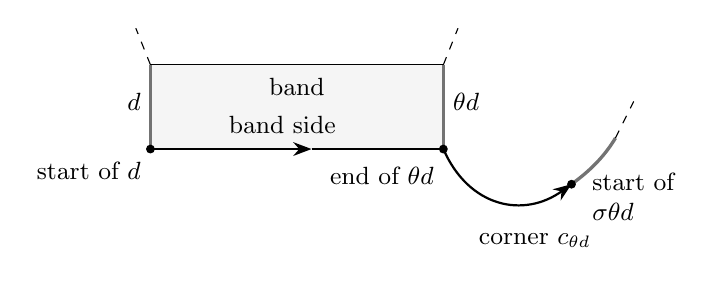
\begin{tikzpicture}[x=0.93cm,y=0.93cm,>=Stealth,
  every node/.style={font=\small}]
  \fill[black!4] (0,0) rectangle (4,1.15);
  \draw (0,1.15)--(4,1.15);
  \draw[very thick,black!55] (0,0)--(0,1.15);
  \draw[very thick,black!55] (4,0)--(4,1.15);
  \draw[->,thick] (0,0)--(2.2,0);
  \draw[thick] (2.2,0)--(4,0);
  \draw[->,thick] (4,0) .. controls (4.35,-0.8) and
    (5.10,-0.95) .. (5.75,-0.48);
  \draw[very thick,black!55] (5.75,-0.48) .. controls
    (6.0,-0.30) and (6.2,-0.10) .. (6.35,0.15);
  \draw[dashed] (4,1.15)--(4.20,1.65);
  \draw[dashed] (6.35,0.15)--(6.60,0.65);
  \draw[dashed] (0,1.15)--(-0.20,1.65);
  \fill (0,0) circle (1.6pt);
  \fill (4,0) circle (1.6pt);
  \fill (5.75,-0.48) circle (1.6pt);
  \node[left] at (0,0.65) {$d$};
  \node[right] at (4,0.65) {$\theta d$};
  \node at (2,0.85) {band};
  \node[above] at (1.8,0.08) {band side};
  \node[below left] at (0,-0.05) {start of $d$};
  \node[below left] at (4,-0.12) {end of $\theta d$};
  \node[below] at (5.25,-1.02) {corner $c_{\theta d}$};
  \node[right,align=left] at (5.9,-0.65)
    {start of\\$\sigma\theta d$};
\end{tikzpicture}
\caption{One boundary step, with the attached slots drawn as thick gray
intervals.  The arrow crosses a band side and then follows the corner
after the partner slot.  This gives the permutation $\sigma\theta$ and
the label $c_{\theta d}$.  The drawing is local: the disk signs and types
are unspecified, and the two band ends may lie on the same disk.}
\label{fig:boundary-step}
\end{figure}

\smallskip\noindent
\emph{Distributing phases among boundary components.}
For any real numbers $(\eta_z)_z$ with $\sum_z\eta_z=0$, we can choose
real numbers $(\gamma_d)_{d\in\mathcal D}$ such that
\begin{equation}\label{eq:boundary-flow}
 \gamma_{\theta d}=-\gamma_d,\qquad
 \sum_{d\in z}\gamma_d=\eta_z.
\end{equation}
To see this, form a graph whose vertices are the boundary cycles and
whose edges are the pairs $\{d,\theta d\}$, with an end incident to the
cycle containing that slot.  Loops and multiple edges are allowed.
Connectedness of $\Sigma$ means that $\sigma$ and $\theta$ act
transitively on $\mathcal D$.  Since $\sigma\theta$ and $\theta$ generate
the same permutation group, this graph is connected.  Choose a spanning
tree and set the values on all other edges to zero.  At a leaf, set the
value at its end of the remaining edge equal to its prescribed sum and
the value at the other end to its negative; remove the leaf and adjust
the prescribed sum at its neighbor.  The zero total ensures the last
vertex is satisfied.  This proves \eqref{eq:boundary-flow}, including
the one-vertex case.

Use the algebra $M_{2b}(\mathcal M)$ of Section~\ref{sec:phase}, acting on
$\mathbb C^{\mathcal D}\otimes\ell^2(G)$, and define
\begin{equation}\label{eq:surface-operators}
 \begin{split}
 S(e_d\otimes v)&=e_{\sigma d}\otimes L(c_d^{-1})v,\\
 \Theta(e_d\otimes v)&=e^{2\pi i\gamma_d}
                      e_{\theta d}\otimes v.
 \end{split}
\end{equation}
Both operators are unitary, and \eqref{eq:boundary-flow} gives
$\Theta^2=I$.  We identify scalar matrices with their tensor products
with the identity on $\ell^2(G)$; their trace $\tau_{2b}$ is therefore
the ordinary matrix trace.

\smallskip\noindent
\emph{The upper phase bound.}
We will choose a scalar unitary involution $J$ and use the factorization
$S\Theta=(SJ)(J\Theta)$.  We arrange that $SJ$ is an involution with
known phase, and use the fixed-space theorem to give $J\Theta$ many
fixed vectors.
For each $i\in I$, order the $k_i$ disks of each sign.  At each position
$t$, their slots form two coordinate spaces, each identified with
$\mathbb C^{k_i}$.  Given $X_i\in\mathrm U(k_i)$, define a scalar unitary
involution $J$ by sending the positive array at $(i,t)$ to the negative
array by $X_i$, and the negative array back by $X_i^{-1}$.
The same $X_i$ is used at every position of type $i$.

The corner conventions give
\begin{equation}\label{eq:reversal-involution}
 JSJ=S^{-1}.
\end{equation}
Indeed, on positive arrays $S$ moves from $t$ to $t+1$ with coefficient
$L(g_{i,t}^{-1})$, whereas on negative arrays it moves from $t$ to
$t-1$ with coefficient $L(g_{i,t-1})$.  Applying $J$ on either side
interchanges these rules; its factors $X_i$ and $X_i^{-1}$ cancel
because the coefficients are constant across each array and commute
with scalar matrices.  Thus $SJ$ is a unitary involution.  It exchanges
the two disk signs, so its diagonal blocks, and hence its trace, are
zero.  Its $-1$ spectral projection $(I-SJ)/2$ has trace $b$, giving
\begin{equation}\label{eq:disk-involution-phase}
 \ell(SJ)=\frac b2.
\end{equation}

We now choose the $X_i$ so that $J\Theta$ has many fixed vectors.  Regroup
the scalar coordinates by variable index $j$ and traversal sign into
spaces $V_{j,+}$ and $V_{j,-}$.  For each occurrence $(i,t)$ with
$\nu_{i,t}=j$, each space has one block of dimension $k_i$: the positive
or negative disk array is selected according to its traversal sign.
In particular both spaces have dimension
\[
 d_j=\sum_{\substack{i\in I,\ 1\leq t\leq N_i\\\nu_{i,t}=j}}k_i,
 \qquad \sum_j d_j=b.
\]
Both $J$ and $\Theta$ exchange $V_{j,+}$ and $V_{j,-}$.  Under the array
coordinates, let $P_j\in\mathrm U(d_j)$ represent
$\Theta:V_{j,+}\longrightarrow V_{j,-}$.  On the return map
$J:V_{j,-}\longrightarrow V_{j,+}$, the block at $(i,t)$ is
$X_i^{-s_{i,t}}$.  Hence
\begin{equation}\label{eq:fixed-space-application}
 (J\Theta)|_{V_{j,+}}
   =\operatorname{diag}_{(i,t):\,\nu_{i,t}=j}
           (X_i^{-s_{i,t}})P_j.
\end{equation}
The signed block counts here are
$\sum_{t:\nu_{i,t}=j}(-s_{i,t})=-a_{ij}$.  The matrix formed by the rows
of $-A$ indexed by $I$ has full row rank, so
Theorem~\ref{thm:fixed-space} supplies $X_i$ for which
\[
 \dim_{\mathbb C}\ker\bigl((J\Theta-I)|_{\bigoplus_j V_{j,+}}\bigr)
 \geq K.
\]
There are equally many fixed vectors on $\bigoplus_jV_{j,-}$: $J$
interchanges the two sums and satisfies
$J(J\Theta)J=(J\Theta)^{-1}$.  Thus the full fixed-space dimension
$f$ of the scalar matrix $J\Theta$ is at least $2K$.
The same conjugacy makes its eigenvalue multiset invariant under
$\lambda\mapsto\lambda^{-1}$.  Since
$h(\lambda)+h(\lambda^{-1})=1$ for $\lambda\ne1$ and is zero at $1$,
\[
 2\ell(J\Theta)=2b-f\leq2b-2K.
\]
Using $S\Theta=(SJ)(J\Theta)$, \eqref{eq:disk-involution-phase} and
Lemma~\ref{lem:phase-subadditivity} now give
\begin{equation}\label{eq:surface-phase-upper}
 \ell(S\Theta)\leq\frac32 b-K.
\end{equation}
This holds for every phase distribution in \eqref{eq:boundary-flow};
the auxiliary choice of $J$ may depend on that distribution.

\smallskip\noindent
\emph{The boundary formula and the cut limit.}
It remains to read the left side of \eqref{eq:surface-phase-upper} from
the boundary.  On the coordinates of a cycle
$z=(d_1,\ldots,d_a)$ of $\sigma\theta$, the operator $S\Theta$ is a
weighted cyclic shift $T_z$ whose step from $d_t$ to $d_{t+1}$ has weight
$e^{2\pi i\gamma_{d_t}}L(c_{\theta d_t}^{-1})$.  The circuit starting
at $d_1$ therefore has weight
\[
 e^{2\pi i\sum_{d\in z}\gamma_d}
 L(c_{\theta d_a}^{-1}\cdots c_{\theta d_1}^{-1})
   =e^{2\pi i\eta_z}L(r_z^{-1}).
\]
Lemma~\ref{lem:cycle-phase} yields the exact formula
\begin{equation}\label{eq:boundary-phase}
 \ell(T_z)=\frac{a(z)-1}{2}
       +\tau\bigl(h(e^{2\pi i\eta_z}L(r_z^{-1}))\bigr).
\end{equation}

Choose the possibly exceptional component $z_0$, and for $\epsilon>0$
set
\[
 \eta_z=-\epsilon\quad(z\ne z_0),\qquad
 \eta_{z_0}=(q-1)\epsilon.
\]
These phases sum to zero, so \eqref{eq:surface-phase-upper} applies.
For $z\ne z_0$, the assumption $r_z=1$ makes the last term of
\eqref{eq:boundary-phase} equal to $1-\epsilon$ when $0<\epsilon<1$.
For $z_0$, the scalar phase approaches zero from the nonnegative side.
Thus $h(e^{2\pi i(q-1)\epsilon}\lambda)\to h(\lambda)$ at every point
of the unit circle, including $\lambda=1$.  Bounded convergence in the
spectral measure gives
\[
 \tau\bigl(h(e^{2\pi i(q-1)\epsilon}L(r_{z_0}^{-1}))\bigr)
 \longrightarrow \tau\bigl(h(L(r_{z_0}^{-1}))\bigr).
\]
This also covers $q=1$, when the scalar phase is identically zero.
Summing \eqref{eq:boundary-phase} over all cycles and using
\eqref{eq:planar-euler}, we obtain
\begin{align*}
 \lim_{\epsilon\downarrow0}\ell(S\Theta)
 &=\frac{2b-q}{2}+q-1+\tau\bigl(h(L(r_{z_0}^{-1}))\bigr)\\
 &=\frac32 b-K+\tau\bigl(h(L(r_{z_0}^{-1}))\bigr).
\end{align*}
The upper bound \eqref{eq:surface-phase-upper} forces the last trace to
be zero.  Faithfulness of $\tau$ and nonnegativity of $h$ imply
$L(r_{z_0}^{-1})=I$.  Applying this operator to $\delta_1$ gives
$r_{z_0}=1$, as required.
\end{proof}

\section{From a kernel relation to a solution}
\label{sec:kernel}

We now apply Proposition~\ref{prop:planar} to prove
Theorem~\ref{thm:main}. The required surfaces must be embedded in a disk:
an arbitrary pairing of variable occurrences would not guarantee
planarity. Following the construction in
\cite[Section~5]{OpenAIKervaire2026}, we obtain the bands as level arcs
of the variable-circle maps on a punctured disk. This also ensures that the coefficient map is
constant along every band.

\subsection{A punctured disk for the relation}

Let $g\in G$ lie in the normal closure of the relators. By definition,
there is a finite expression in $G*F_n$
\begin{equation}\label{eq:normal-product}
 g=\prod_{\alpha=1}^{u}
       b_\alpha w_{i_\alpha}^{\epsilon_\alpha}b_\alpha^{-1},
 \qquad b_\alpha\in G*F_n,\qquad\epsilon_\alpha\in\{1,-1\}.
\end{equation}
If $u=0$, then $g=1$. Assume $u>0$. Use the cyclic representatives
of the relators chosen in Section~\ref{sec:planar}; conjugating a
relator only changes the corresponding conjugators in
\eqref{eq:normal-product}.

Choose a based CW presentation space $Y$ with $\pi_1(Y)=G$, and put
\[
 Y'=Y\vee S^1_1\vee\cdots\vee S^1_n.
\]
The added circles represent the variables, so $\pi_1(Y')=G*F_n$.
Choose based loops in $Y$ for the coefficients and for $g$. No
asphericity or finiteness property of $Y$ is needed.

Let $\Delta$ be an oriented polygonal disk and remove the interiors
of $u$ disjoint polygonal disks $D_\alpha$ in its interior. On the
resulting punctured disk
\[
 P=\Delta\setminus\bigcup_{\alpha=1}^{u}\operatorname{int}D_\alpha
\]
there is a map $f:P\to Y'$ with these boundary values: the outer
boundary reads $g$ in $Y$, and $\partial D_\alpha$, oriented as the
boundary of the missing disk, reads
$w_{i_\alpha}^{\epsilon_\alpha}$. Each variable letter is represented
by one monotone traversal of its circle. The intervening coefficient
intervals are mapped to the chosen loops in $Y$; retain an interval
even when its label is the identity.

Here is an explicit reason that these values extend over $P$. Cut $P$
along disjoint arcs from the outer boundary to the holes, and map those
arcs to the loops for $b_\alpha$. Place their outer endpoints in a
constant portion of the outer loop, with the holes encountered in reverse
order after the outer traversal. The boundary of the cut disk reads
\[
 g\bigl(b_u w_{i_u}^{\epsilon_u}b_u^{-1}\bigr)^{-1}
  \cdots
  \bigl(b_1 w_{i_1}^{\epsilon_1}b_1^{-1}\bigr)^{-1}.
\]
It is nullhomotopic by \eqref{eq:normal-product}. A nullhomotopy
extends the map across the cut disk. The two copies of each cut arc
have the same map with opposite traversal, so the extension descends
to $P$. Notice that the induced boundary orientation of $P$ on a hole
is opposite to the missing-disk orientation; this explains the inverses
in the displayed word.

\subsection{Disjoint bands from circle levels}

Let $f_j:P\to S^1_j=\mathbb R/\mathbb Z$ be the projection of $f$
that collapses all the other wedge summands, and let $v:P\to Y$ be
the coefficient projection. We construct bands on which $v$ is exactly
constant, without changing the boundary values of any $f_j$.

Choose a common sufficiently fine finite triangulation of $P$ and
piecewise affine circle maps $\widetilde f_j$ satisfying
\[
 \widetilde f_j|_{\partial P}=f_j|_{\partial P},
 \qquad
 \operatorname{dist}(\widetilde f_j(p),f_j(p))<\frac1{12}
 \quad(p\in P).
\]
These approximations can be constructed directly. The boundary maps are
already piecewise affine in the angular coordinate. Subdivide to respect
their breakpoints and so finely that the image of each triangle under
each $f_j$ lies in a short arc of the circle. Lift that arc to $\mathbb R$
and interpolate its vertex values. The lifts on a shared edge differ
by an integer, so the interpolants agree as circle maps. Uniform
continuity gives the stated error bound.

For each $j$, choose $t_j\in(1/3,2/3)$ that is not the image of any
vertex under $\widetilde f_j$. The level set
$\widetilde f_j^{-1}(t_j)$ is a finite disjoint union of polygonal
circles and properly embedded polygonal arcs. On each triangle it
consists of line segments, and avoidance of vertices makes the segments
join without branching. Since the approximation is fixed on the
boundary, there is exactly one endpoint for each occurrence of
$x_j^{\pm1}$ on a hole and no endpoint on the outer boundary or on a
coefficient interval.

These level sets are disjoint for different indices. Indeed, at a point
of $\widetilde f_j^{-1}(t_j)$ the original $f_j$ is at distance more
than $1/4$ from the circle basepoint. Thus $f$ lands in the $j$th
variable circle away from the wedge point, and all its other circle
projections vanish. The same remains true in a neighborhood of the
level set. In particular, $v$ is constant at the basepoint on that
neighborhood. This argument uses the original wedge-valued map $f$;
the separately approximated maps need not themselves combine to a map
into the wedge.

Discard the closed level curves and choose thin, mutually disjoint
rectangular neighborhoods of the proper arcs inside these neighborhoods.
They are the bands. Each meets the holes in small intervals inside the
corresponding variable traversals, and every occurrence has exactly one
such interval. Coorientation of a circle level makes the two endpoint
crossing signs of an arc opposite with respect to the boundary
orientation of $P$. Reversing both orientations to the missing-disk
orientations leaves the signs opposite. Hence each band pairs the same
variable with opposite traversal signs, as required in
Proposition~\ref{prop:planar}.

Use the smaller attachment intervals as the slots. The pieces of a
variable traversal outside its slot project constantly to $Y$, so
shrinking the slots does not change any coefficient label between them.
Moreover, $v$ is constant on every band. Reinsert the disks $D_\alpha$
as the signed word disks. Their union with the bands is a compact
surface embedded in the interior of $\Delta$, with every slot paired.
Every connected component is planar, and its boundary words are exactly
the loops supplied by $v$ on those boundary circles.

\subsection{Filling from the inside out}

It remains to account for the possibility of several components nested
inside one another. Each connected component has one exterior boundary
circle whose Jordan disk contains the component; its other boundary
circles enclose the inner complementary disks. The exterior Jordan
disks of distinct components are disjoint or nested. Choose a component
whose exterior disk is minimal under inclusion. Its inner complementary
disks contain no other component, and hence contain no missing word disk.
The coefficient map $v$ is already defined on each of them. Their
boundary words are therefore trivial in $G$.

Proposition~\ref{prop:planar} now implies that the exterior boundary
word of the chosen component is also trivial. Its exact boundary loop
extends to a map of its Jordan disk into $Y$. Replace $v$ inside that
disk by this extension. The two maps agree on the boundary, so they
paste continuously. No other component lies in the disk, and the
coefficient labels and band constants on all remaining components are
unchanged.

Repeating this finite procedure removes all components. The result is
a map $\Delta\to Y$ extending the original outer loop for $g$.
Consequently $g=1$ in $G$. This proves the injectivity in
Theorem~\ref{thm:main}; its quotient supplies the simultaneous solution.
\qed

\begin{remark}\label{rem:infinite-systems}
The finite statement also implies the version with arbitrary sets of
variables and equations. Assume the exponent rows, each of finite
support, are linearly independent over $\mathbb Q$. Any element of
$G$ killed in the quotient has a normal-closure expression involving
only finitely many relators and finitely many variables, including those
in its conjugators. The corresponding finite exponent matrix still has
independent rows, so Theorem~\ref{thm:main} makes that element trivial.
\end{remark}

\begin{thebibliography}{99}

\bibitem{AntezanaLarotondaVarela2012}
J.~Antezana, G.~Larotonda, and A.~Varela,
\emph{Thompson-type formulae},
J. Funct. Anal. \textbf{262} (2012), no.~4, 1515--1528.
\href{https://doi.org/10.1016/j.jfa.2011.11.011}{doi:10.1016/j.jfa.2011.11.011}.

\bibitem{Borel1953}
A.~Borel,
\emph{Sur la cohomologie des espaces fibr\'es principaux et des espaces
homog\`enes de groupes de Lie compacts},
Ann. of Math. (2) \textbf{57} (1953), no.~1, 115--207.
\href{https://doi.org/10.2307/1969728}{doi:10.2307/1969728}.

\bibitem{Chen2026}
L.~Chen,
\emph{The Kervaire conjecture and the minimal complexity of surfaces},
Trans. Amer. Math. Soc. \textbf{379} (2026), 587--626.
\href{https://arxiv.org/abs/2302.09811}{arXiv:2302.09811}.

\bibitem{GerstenhaberRothaus1962}
M.~Gerstenhaber and O.~S.~Rothaus,
\emph{The solution of sets of equations in groups},
Proc. Nat. Acad. Sci. U.S.A. \textbf{48} (1962), no.~9, 1531--1533.
\href{https://doi.org/10.1073/pnas.48.9.1531}{doi:10.1073/pnas.48.9.1531}.

\bibitem{Hatcher2002}
A.~Hatcher,
\emph{Algebraic Topology},
Cambridge University Press, Cambridge, 2002.

\bibitem{Howie1981}
J.~Howie,
\emph{On pairs of $2$-complexes and systems of equations over groups},
J. Reine Angew. Math. \textbf{324} (1981), 165--174.
\href{https://doi.org/10.1515/crll.1981.324.165}{doi:10.1515/crll.1981.324.165}.

\bibitem{Jones2009}
V.~F.~R.~Jones,
\emph{Von Neumann Algebras},
lecture notes, 1 October 2009.
\url{https://math.berkeley.edu/~vfr/VonNeumann2009.pdf}.

\bibitem{Klyachko1993}
A.~A.~Klyachko,
\emph{A funny property of sphere and equations over groups},
Comm. Algebra \textbf{21} (1993), no.~7, 2555--2575.
\href{https://doi.org/10.1080/00927879308824692}{doi:10.1080/00927879308824692}.

\bibitem{KlyachkoMikheenkoRomankov2024}
A.~A.~Klyachko, M.~A.~Mikheenko, and V.~A.~Roman'kov,
\emph{Equations over solvable groups},
J. Algebra \textbf{638} (2024), 739--750.
\href{https://doi.org/10.1016/j.jalgebra.2023.10.004}{doi:10.1016/j.jalgebra.2023.10.004}.

\bibitem{McCleary2001}
J.~McCleary,
\emph{A User's Guide to Spectral Sequences},
second ed., Cambridge Studies in Advanced Mathematics, vol.~58,
Cambridge University Press, Cambridge, 2001.

\bibitem{Nicolaescu2010}
L.~I.~Nicolaescu,
\emph{Schubert calculus on the Grassmannian of hermitian lagrangian spaces},
Adv. Math. \textbf{224} (2010), no.~6, 2361--2434.
\href{https://doi.org/10.1016/j.aim.2010.02.003}{doi:10.1016/j.aim.2010.02.003}.

\bibitem{NitscheThom2022}
M.~Nitsche and A.~Thom,
\emph{Universal solvability of group equations},
J. Group Theory \textbf{25} (2022), no.~1, 1--10.
\href{https://doi.org/10.1515/jgth-2019-0167}{doi:10.1515/jgth-2019-0167}.

\bibitem{OpenAIKervaire2026}
OpenAI,
\emph{The Kervaire theorem for groups},
OpenAI Math Release preprint
\href{https://github.com/openai/math/blob/main/preprints/The-Kervaire-Theorem-for-Groups-September-24-2026/The-Kervaire-Theorem-for-Groups-September-24-2026.pdf}{OAI:The-Kervaire-Theorem-for-Groups-September-24-2026},
2026.

\bibitem{Pestov2008}
V.~G.~Pestov,
\emph{Hyperlinear and sofic groups: a brief guide},
Bull. Symbolic Logic \textbf{14} (2008), no.~4, 449--480.
\href{https://arxiv.org/abs/0804.3968}{arXiv:0804.3968}.

\bibitem{RamirezCoteWise2025}
A.~Ramirez-C\^ot\'e and D.~T.~Wise,
\emph{The Kervaire conjecture via Banach fixed points in power series groups},
Math. Z. \textbf{311} (2025), article~6.
\href{https://doi.org/10.1007/s00209-025-03753-3}{doi:10.1007/s00209-025-03753-3}.

\bibitem{Thompson1986}
R.~C.~Thompson,
\emph{Proof of a conjectured exponential formula},
Linear Multilinear Algebra \textbf{19} (1986), no.~2, 187--197.
\href{https://doi.org/10.1080/03081088608817715}{doi:10.1080/03081088608817715}.

\end{thebibliography}

\end{document}
